\chapter[Realizace skriptů v jazyce Python 3]{Realizace skriptů\\ v jazyce Python 3}

\section{Vytvoření archivu dat TLE}
  Vytvoření lokální databázi dat TLE je nezbytné pro správnou korekci dopplerovského posuvu. Pro umělé družice NO-83 a NO-84 jsou veřejně přístupné data TLE na stránce organizace \zkratka{AMSAT}: <\url{http://amsat.org/pipermail/keps/}>. Tyto data jsou distribuované formou elektronického mailing list, kterého archív se nachází na výše zmíněném URL v jedním souboru. Aby bylo možné použit údaje TLE obsáhnuty v tomhle archivním souboru, je nutné provést extrakci dat TLE dle datu jejího vzniku.

  Na obrázku \ref{fig:TLE_flow} je uveden vývojový diagram skriptu pro extrahování dat TLE. Jako povinný vstupní parametr je název souboru staženého z webové stránky oragnizace \zkratka{AMSAT}. Data TLE jsou posílané v jednom emailu. Skript identifikuje začátek i konec balíků dat TLE. Na začátku každého balíku se hledjí vzory:\\
  \texttt{SB\textbackslash s+KEPS\textbackslash s+@\textbackslash s+AMSAT\textbackslash s+\$ORB\textbackslash d{5}\textbackslash.[A-Z]}\\
  \texttt{\textasciicircum 2Line}\\
  pomocí nástroje na vyhledávání regulárních výrazů implementovaného modulem re ze standardní knihovny jazyka Python. Konec bálíka je značen řetězcem
  \texttt{\textbackslash EX}.

  V případě, že skript narazí na hledaný výraz, nastaví se příslušný příznak. Tyto příznaky zaručí, aby řádky jednoho balíku se připojili k jednomu řetězci. Když skript identifikuje poslední řádek, pospojovaný řetězec řádků se připojí k množině všech balíků TLE dat. Návratovou hodnotou je právě tato množina. Množina v jazyce Python 3 zaručuje jedinečnost všech prvků, obdobně jako množiny z teorie množin.

  K výpisu souboru patří funkce \texttt{dump\_to\_file} skriptu \texttt{TLE.py}. Tato funkce má jeden povinný parametr, množinu dat TLE. Z této množiny se načte každý jeden prvek. V těchto prvcích se prohledává datum vzniku, což se použije jako název souboru. Následně se dle potřeby vytvoří adresář, kterého název je rok vzniku TLE dat. Před vytvářením adresáře se kontroluje přítomnost adresáře, nebo souboru stejného jména, jaký se chystá být vytvořit. Jestli adresář se stejným jménem existuje, začne se de ní zapisovat. V opačném případě předpokládáme, že v adresáři je soubor se stejný jménem musíme název složky, kterou se chystáme vytvořit změnit z důvodu nemožnosti koexistence souboru a adresáře stejného jména v rodičovském adresáři. K názvu složky se přidává znak podtržítka a číslo, které se iteruje inkrementací do doby, kdy v rodičovském se nebude nacházet soubor se stejným jménem. V případě adresáře se stejným jménem nalezeného po přidání dodatečných znaků k názvu souboru, se adresář začne používat k uložení souborů. Čtení z množiny je realizováno pomocí iterací nad její prvkami.

%  ../../Python3/TLE.py
  \begin{figure}[ht]
    \centering
    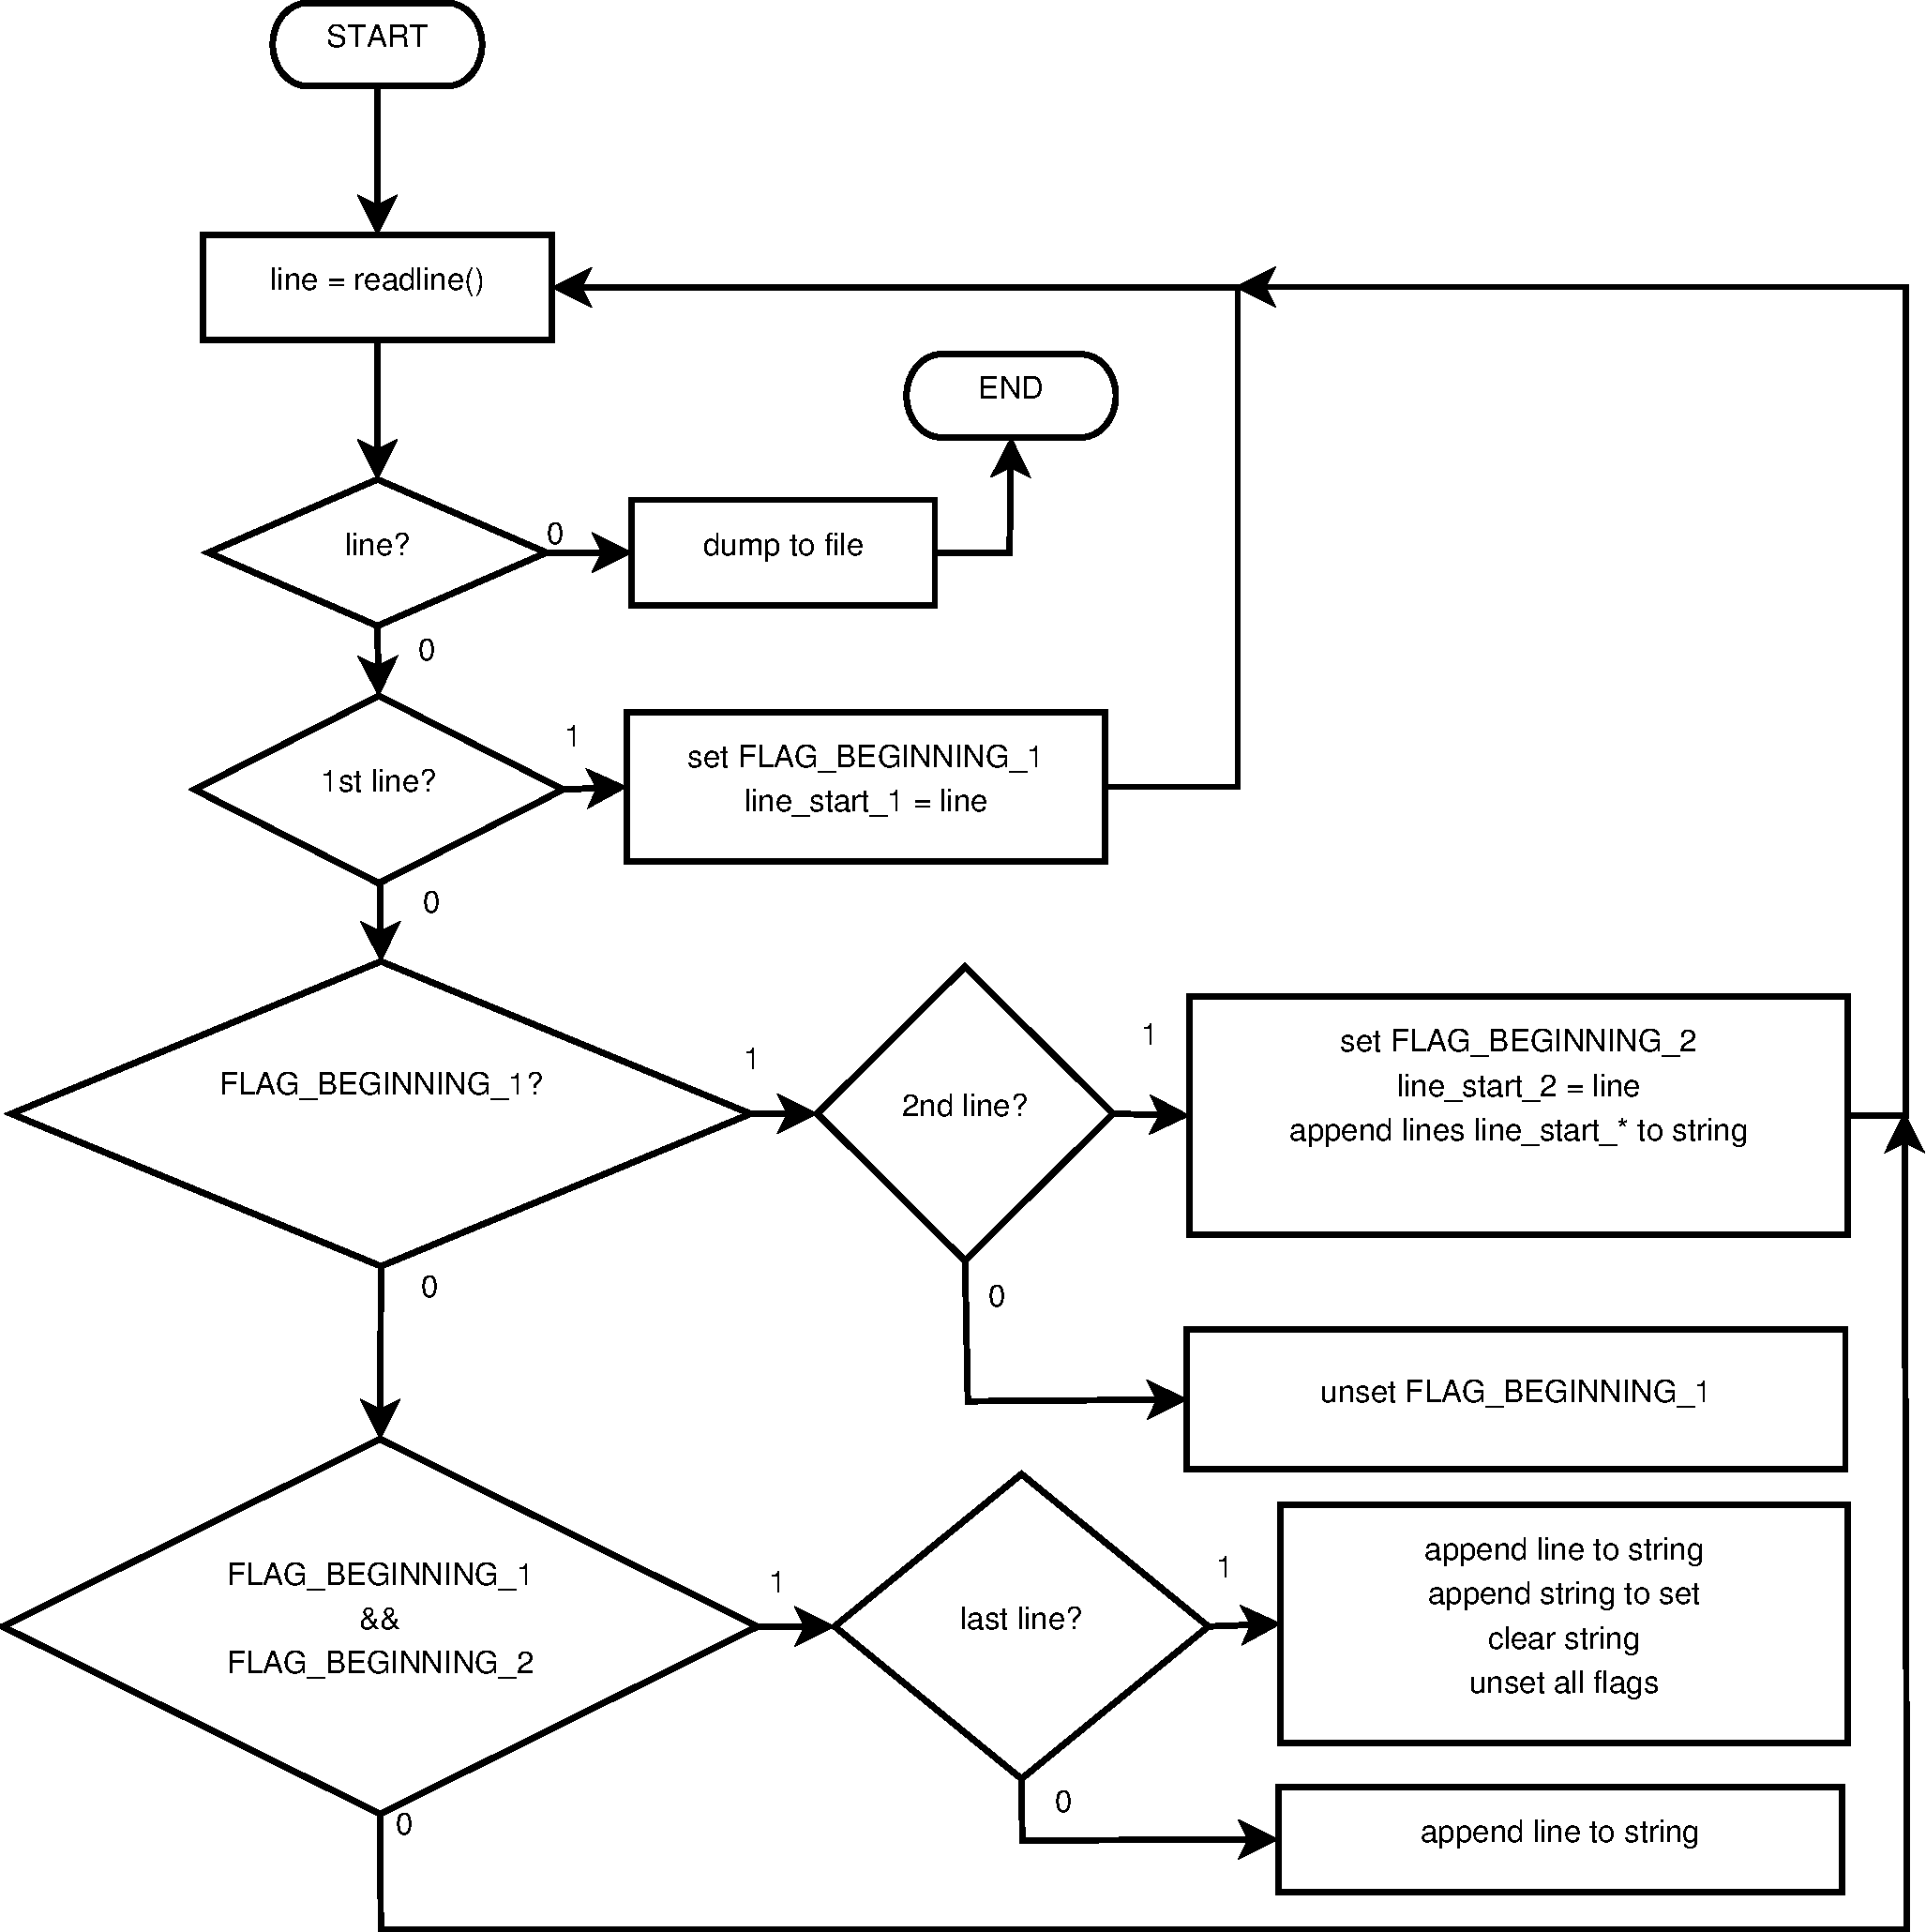
\includegraphics[width=0.98\textwidth]{./obrazky/TLE.pdf}
    \caption{Vývojový diagram extrahování dat TLE}
    \label{fig:TLE_flow}
  \end{figure}

\section{Korekce dopplerovského posuvu}
% gpredict -- libgpredict, doppler
% mediainfo, sox
  Po úspěšném získání nutných souborů s daty TLE pro umělé družice našeho zájmu, můžeme přistoupit ke korekci dopplerovského posuvu signálu, kterou provedeme pomocí programu doppler volně dostupného z repozitáře GIT týmu codehub dostupného na URL <\url{https://github.com/cubehub}>.

  Program doppler je utlitou příkazového řádku, který ze standardního vstupu čte IQ (in-phase, quadrature) data a zpracovává dle zadaných parametrů. Rozlišujeme dva režimy korekce frekvenčního posuvu. V režimu \emph{const} se kompenzuje konstantní posuv kmitočtu, kým v režimu \emph{track} se provádí korekce sledováním pohybu umělé družice a to i dodatečně v případě zpracování předem zaznamenaných dat IQ. V pozdním případě se programu doppler musí předát argument datu a času záznamu ve formátu ISO 8601 \cite{wiki:timeISO} \cite{github:doppler} bez udání časového posuvu v čase UTC.

  Korekce dopplerovského posuvu se provádí programem doppler za pomoci volně dostupné knihovny libgpredict, který je založen na predikčním kódu programu Gpredict. \cite{github:libgpredict}

  Aby se zjednodušilo zpracování velikého množství souborů, byl vytvořen skript v jazyce Python 3 pro automatické zpracování záznamů s IQ daty. Modul get\_undopplred má definovanou funkci undoppler\_it, který jako vstupní parametry má:
  \begin{itemize}
    \item název souboru IQ dat
    \item název družice v notaci OSCAR\footnote{v našém případě se jedná o NO-83, NO-84}
    \item kmitočet na kterém je z družice vysíláno
    \item adresář s IQ daty
    \item adresář s TLE daty
    \item lokace pozemní stanice
  \end{itemize}

  Pomocí těchto údajů se sestrojí řetězec obsahující příkaz shellu BASH, kde jednotlivé příkazy jsou řazeny do tzv. kolony. Jde o zřetězení příkazů oddělených metaznakem svislá čára '|'. Standardní výstup příkazu se předává standardnímu příkazu následujícímu. \cite{book:Brandejs-unix-linux}

  Parametry záznamu IQ dat se zjišťují pomocí modulu pymediainfo, který je tzv. wrapper function knihovny Mediainfo \cite{github:pymediainfo}. Pomocí tohoto modelu lze zjistit kmitočet vzorkování, bitovou hloubku, kódování, počet kanálů, kodek.

  Aby jsme mohli soubory formátu \zkratka{WAV} použít jako vstupní data pro program doppler, je nutné provést změnu formátu dle očekávání programu. K této úloze se použije volný program \zkratka{sox}. Podobně na výstupu lze použít \zkratka{sox} pro převod z RAW Audio formátu na \zkratka{WAV}.

  \begin{figure}[ht]
    \centering
    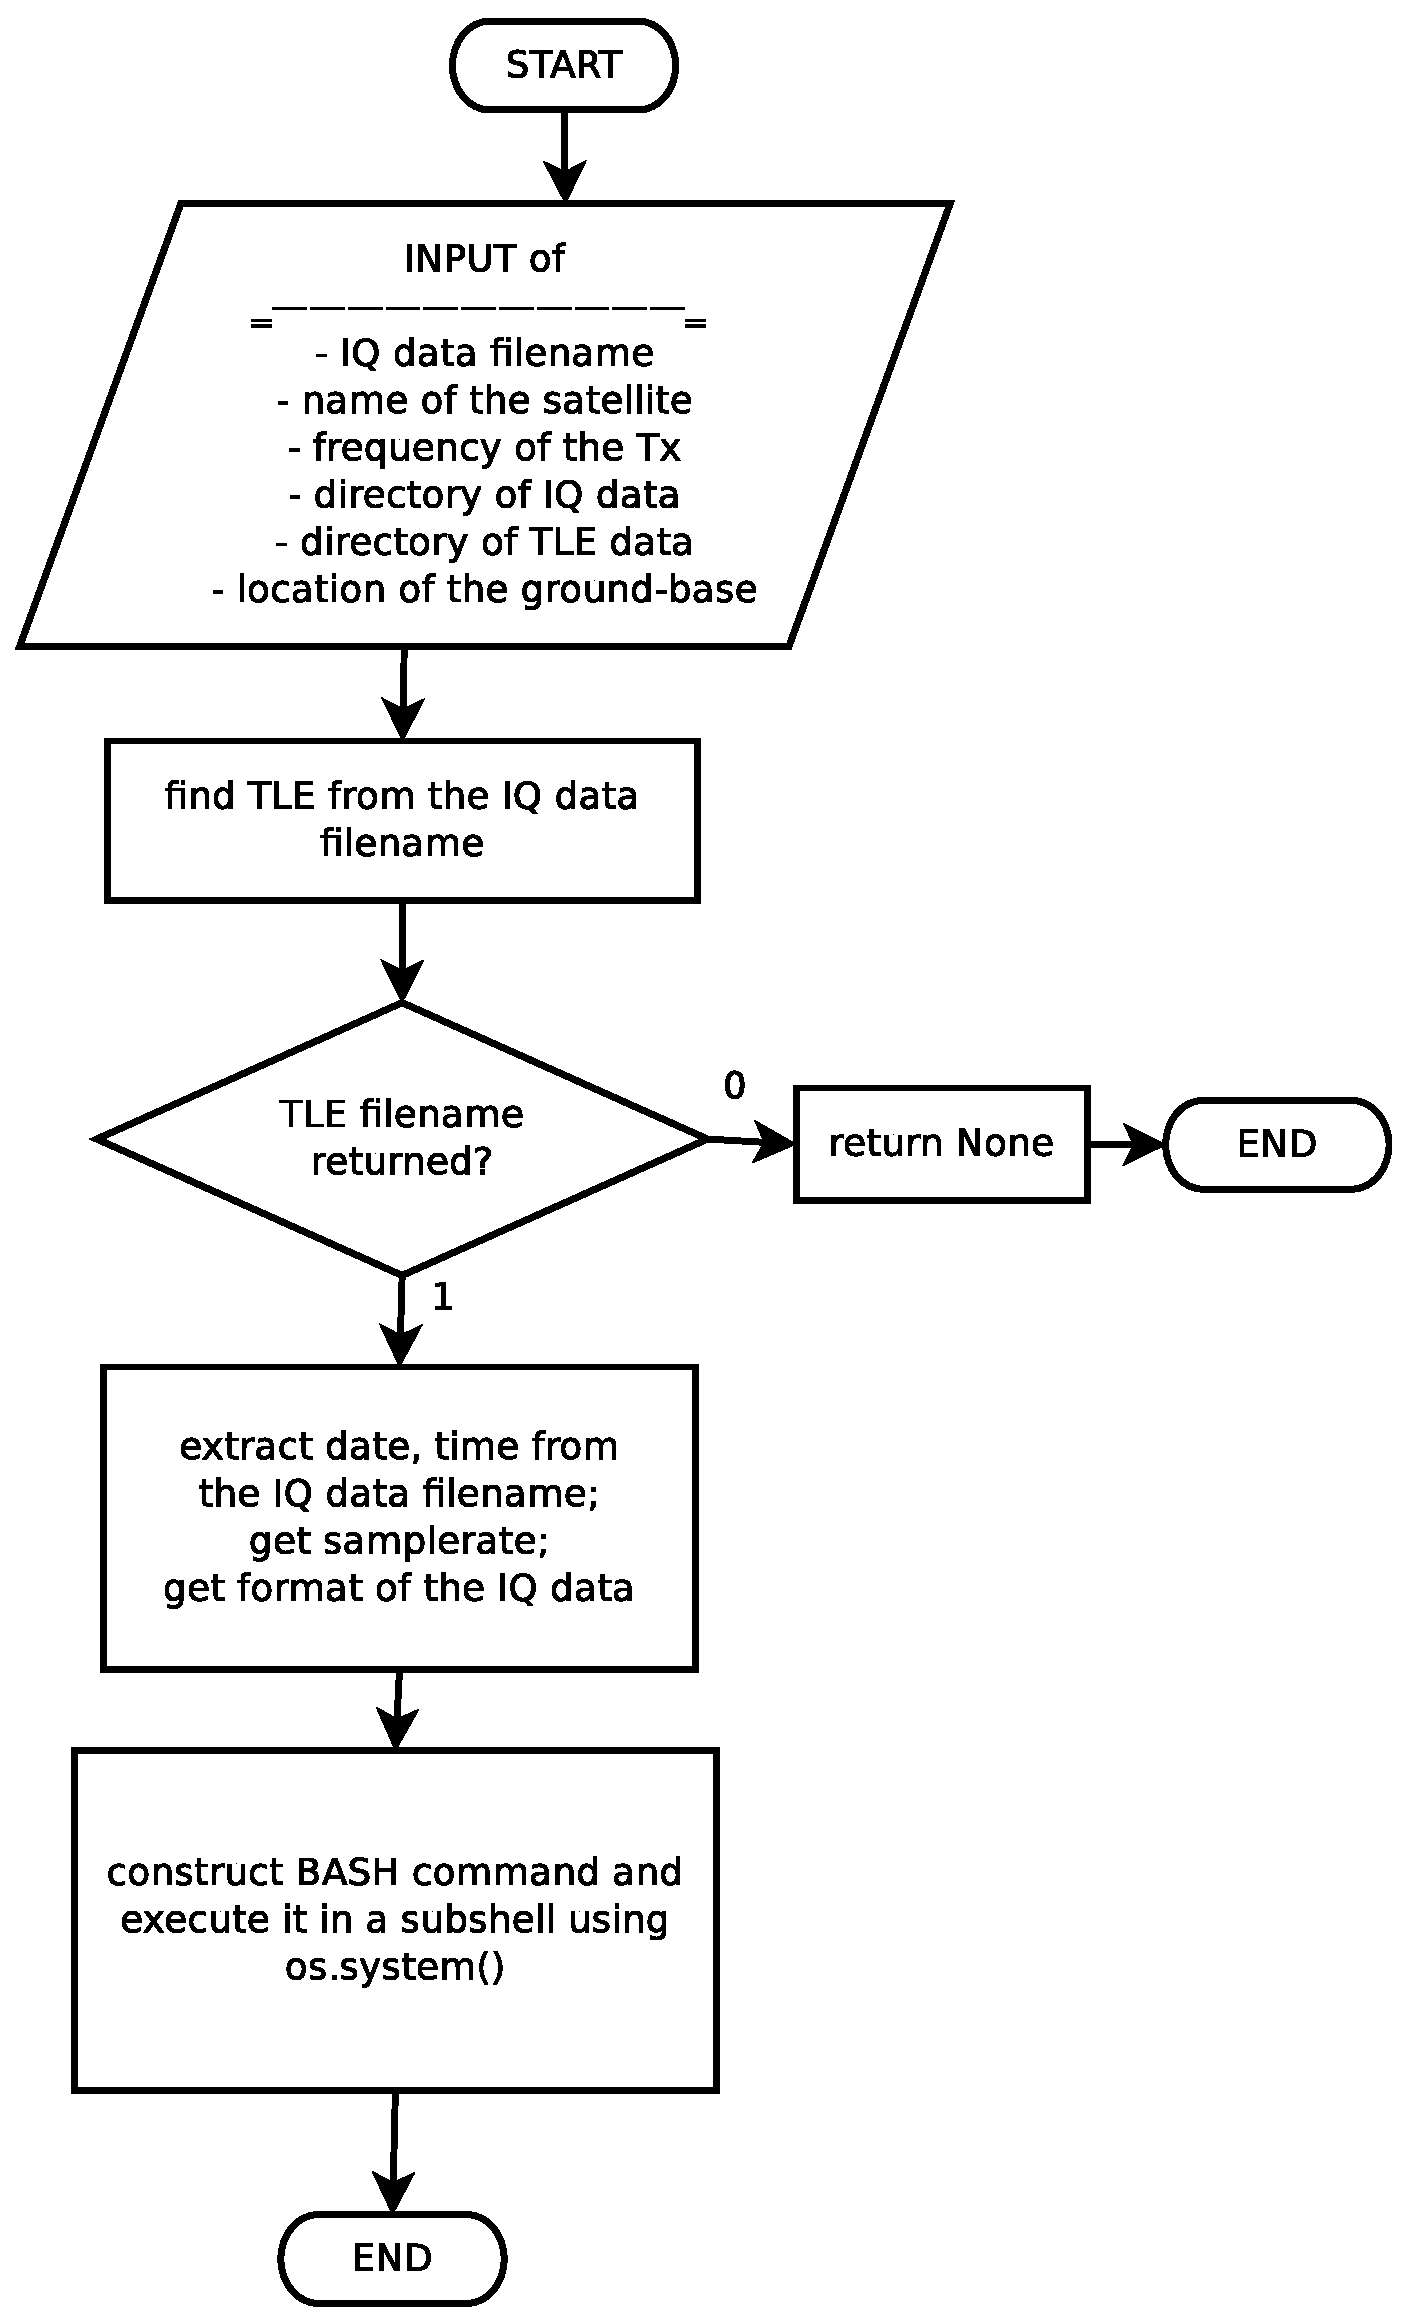
\includegraphics[width=0.65\textwidth]{./obrazky/get_undopplered.eps}
    \caption{Náčrt fungování modulu pro korekci dopplerovho posuvu}
    \label{fig:undoppler}
  \end{figure}

\section{Tvorba spektrogramů}

Kontrola správnosti korekci dopplerovského posuvu lze hrubě odhadnout pomocí spektrogramu korigovaných IQ dat. Pro automatizovaní tohoto procesu slouží modul wav2spectrogram.

Hlavní částí tohoto modulu je funkce IQ\_to\_spectrogram.
Python 3 modul pro tvorbu spektrogramů. Jediným argumentem je název souboru IQ dat. Ostatní parametry jsou buď napevno dány, nebo automaticky zjištění ze souboru IQ dat. Spektrogram je uložen ve formátu \zkratka{PNG}.

\section{Quo vadis moduly?}

Kudy směrují tyto moduly? Je filozofická otázka, na kterou by se dalo napsat nespočetné množství stran. Lze říct, že sami o sobě tyto moduly, skripty, neprovádějí automatické zpracování signálů, avšak jako základ pro budoucí vývoj mohou být nápomocné pro svou vlastnost zjednodušeného volání jinou funkcí, skriptem. Jazyk Python umožňuje jednoduchou iteraci nad všemi soubory složky, což nám dává možnost dávkového zpracování souborů s IQ daty.

Do budoucna se počítá s dalším zpracováním frekvenčně zkorigovaných signálů -- demodulace FM a následné dekódování přijatých zpráv telemetrie PSK31.


\chapter{Prezentace výsledků}
\label{chap:prez}

Funkčnost skript bylo ověřeno na záznamech signálů umělých družic NO-83, a NO-84.

Na obrázku \ref{fig:NO-84_raw} je znázorněn spektrogram přijatého rádiového signálu umělé družice NO-84. Dopplerův efekt lze zpozorovat na základě zjevného klesání kmitočtu přijatého signálu v závislosti na čase. Za předpokladu konstantního kmitočtu nosné vysílače a kmitočtu lokálního oscilátoru směšovače radiového přijímače můžeme usoudit, že umělá družice se k nám přibližuje a její relatívní rychlost vzhledem ke místu příjmu se zmenšuje.

Po aplikování korekci dopplerovského posuvu je spektrogram signálu znázorněn na obrázku \ref{fig:NO-84_ud}. Vidno, že drift kmitočtu od ideálního stavu přímky je minimální. Tyto odchylky jsou dány:

\begin{itemize}
  \item nepřesnost lokálního oscilátoru družice
  \item korekce kmitočtového posuvu po částech signálu diskrétní časové délky
  \item nepřesnost modelu SGP4 při předvídání pohybu družice
\end{itemize}

\begin{figure}[ht]
  \centering
  \includegraphics[width=0.9\textwidth]{./obrazky/HDSDR_20160123_152139Z_435320kHz_RF.png}
  \caption{Spektrogram signálu družice NO-84 bez korekce}
  \label{fig:NO-84_raw}
\end{figure}

\begin{figure}[ht]
  \centering
  \includegraphics[width=0.9\textwidth]{./obrazky/HDSDR_20160123_152139Z_435320kHz_RFUD.png}
  \caption{Spektrogram signálu družice NO-84 s korekcí}
  \label{fig:NO-84_ud}
\end{figure}

\begin{figure}[ht]
  \centering
  \includegraphics[width=0.9\textwidth]{./obrazky/HDSDR_20160127_161858Z_435320kHz_RF.png}
  \caption{Spektrogram signálu družice NO-83 bez korekce}
  \label{fig:NO-83_raw}
\end{figure}

\begin{figure}[ht]
  \centering
  \includegraphics[width=0.9\textwidth]{./obrazky/HDSDR_20160127_161858Z_435320kHz_RFUD.png}
  \caption{Spektrogram signálu družice NO-83 s korekcí}
  \label{fig:NO-83_ud}
\end{figure}
